\begin{table}
    \centering
    \begin{tabular}{cccc}
        \textbf{Shape (House)} &
        \textbf{Community} &
        \textbf{Grid} &
        \textbf{Cycle}\\
        \midrule
        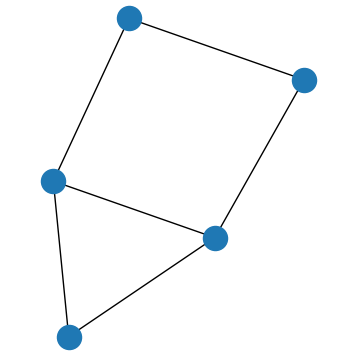
\includegraphics[width=0.15\textwidth]{figures/house.png} &
        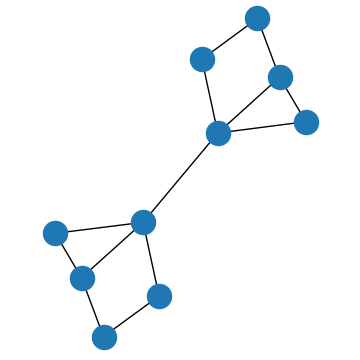
\includegraphics[width=0.15\textwidth]{figures/community.png} &
        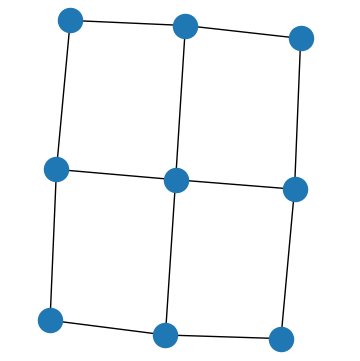
\includegraphics[width=0.15\textwidth]{figures/grid.png} &
        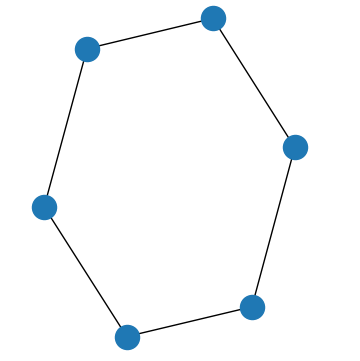
\includegraphics[width=0.15\textwidth]{figures/cycle.png} \\
    \end{tabular}
    \caption{The four different motifs used by the synthetic datasets. Each motif is attached to a specific base graph. Note that the community motif is created by combining two different shape motif graphs.}
    \label{tab:motifs}
\end{table}

